\documentclass[twoside]{book}

% Packages required by doxygen
\usepackage{calc}
\usepackage{doxygen}
\usepackage{graphicx}
\usepackage[utf8]{inputenc}
\usepackage{makeidx}
\usepackage{multicol}
\usepackage{multirow}
\usepackage{textcomp}
\usepackage[table]{xcolor}

% Font selection
\usepackage[T1]{fontenc}
\usepackage{mathptmx}
\usepackage[scaled=.90]{helvet}
\usepackage{courier}
\usepackage{amssymb}
\usepackage{sectsty}
\renewcommand{\familydefault}{\sfdefault}
\allsectionsfont{%
  \fontseries{bc}\selectfont%
  \color{darkgray}%
}
\renewcommand{\DoxyLabelFont}{%
  \fontseries{bc}\selectfont%
  \color{darkgray}%
}

% Page & text layout
\usepackage{geometry}
\geometry{%
  a4paper,%
  top=2.5cm,%
  bottom=2.5cm,%
  left=2.5cm,%
  right=2.5cm%
}
\tolerance=750
\hfuzz=15pt
\hbadness=750
\setlength{\emergencystretch}{15pt}
\setlength{\parindent}{0cm}
\setlength{\parskip}{0.2cm}
\makeatletter
\renewcommand{\paragraph}{%
  \@startsection{paragraph}{4}{0ex}{-1.0ex}{1.0ex}{%
    \normalfont\normalsize\bfseries\SS@parafont%
  }%
}
\renewcommand{\subparagraph}{%
  \@startsection{subparagraph}{5}{0ex}{-1.0ex}{1.0ex}{%
    \normalfont\normalsize\bfseries\SS@subparafont%
  }%
}
\makeatother

% Headers & footers
\usepackage{fancyhdr}
\pagestyle{fancyplain}
\fancyhead[LE]{\fancyplain{}{\bfseries\thepage}}
\fancyhead[CE]{\fancyplain{}{}}
\fancyhead[RE]{\fancyplain{}{\bfseries\leftmark}}
\fancyhead[LO]{\fancyplain{}{\bfseries\rightmark}}
\fancyhead[CO]{\fancyplain{}{}}
\fancyhead[RO]{\fancyplain{}{\bfseries\thepage}}
\fancyfoot[LE]{\fancyplain{}{}}
\fancyfoot[CE]{\fancyplain{}{}}
\fancyfoot[RE]{\fancyplain{}{\bfseries\scriptsize Generated on Wed Jan 31 2018 17\-:14\-:27 for Q\-D\-S\-P by Doxygen }}
\fancyfoot[LO]{\fancyplain{}{\bfseries\scriptsize Generated on Wed Jan 31 2018 17\-:14\-:27 for Q\-D\-S\-P by Doxygen }}
\fancyfoot[CO]{\fancyplain{}{}}
\fancyfoot[RO]{\fancyplain{}{}}
\renewcommand{\footrulewidth}{0.4pt}
\renewcommand{\chaptermark}[1]{%
  \markboth{#1}{}%
}
\renewcommand{\sectionmark}[1]{%
  \markright{\thesection\ #1}%
}

% Indices & bibliography
\usepackage{natbib}
\usepackage[titles]{tocloft}
\setcounter{tocdepth}{3}
\setcounter{secnumdepth}{5}
\makeindex

% Hyperlinks (required, but should be loaded last)
\usepackage{ifpdf}
\ifpdf
  \usepackage[pdftex,pagebackref=true]{hyperref}
\else
  \usepackage[ps2pdf,pagebackref=true]{hyperref}
\fi
\hypersetup{%
  colorlinks=true,%
  linkcolor=blue,%
  citecolor=blue,%
  unicode%
}

% Custom commands
\newcommand{\clearemptydoublepage}{%
  \newpage{\pagestyle{empty}\cleardoublepage}%
}


%===== C O N T E N T S =====

\begin{document}

% Titlepage & ToC
\hypersetup{pageanchor=false}
\pagenumbering{roman}
\begin{titlepage}
\vspace*{7cm}
\begin{center}%
{\Large Q\-D\-S\-P }\\
\vspace*{1cm}
{\large Generated by Doxygen 1.8.6}\\
\vspace*{0.5cm}
{\small Wed Jan 31 2018 17:14:27}\\
\end{center}
\end{titlepage}
\clearemptydoublepage
\tableofcontents
\clearemptydoublepage
\pagenumbering{arabic}
\hypersetup{pageanchor=true}

%--- Begin generated contents ---
\chapter{Data Structure Index}
\section{Data Structures}
Here are the data structures with brief descriptions\-:\begin{DoxyCompactList}
\item\contentsline{section}{\hyperlink{classqdsp__interface}{qdsp\-\_\-interface} }{\pageref{classqdsp__interface}}{}
\item\contentsline{section}{\hyperlink{interfaceqdsp__interface_1_1qdspInit}{qdsp\-\_\-interface\-::qdsp\-Init} }{\pageref{interfaceqdsp__interface_1_1qdspInit}}{}
\item\contentsline{section}{\hyperlink{structQDSPplot}{Q\-D\-S\-Pplot} }{\pageref{structQDSPplot}}{}
\item\contentsline{section}{\hyperlink{interfaceqdsp__interface_1_1qdspSetBGColor}{qdsp\-\_\-interface\-::qdsp\-Set\-B\-G\-Color} }{\pageref{interfaceqdsp__interface_1_1qdspSetBGColor}}{}
\item\contentsline{section}{\hyperlink{interfaceqdsp__interface_1_1qdspSetBounds}{qdsp\-\_\-interface\-::qdsp\-Set\-Bounds} }{\pageref{interfaceqdsp__interface_1_1qdspSetBounds}}{}
\item\contentsline{section}{\hyperlink{interfaceqdsp__interface_1_1qdspSetGridX}{qdsp\-\_\-interface\-::qdsp\-Set\-Grid\-X} }{\pageref{interfaceqdsp__interface_1_1qdspSetGridX}}{}
\item\contentsline{section}{\hyperlink{interfaceqdsp__interface_1_1qdspSetGridY}{qdsp\-\_\-interface\-::qdsp\-Set\-Grid\-Y} }{\pageref{interfaceqdsp__interface_1_1qdspSetGridY}}{}
\item\contentsline{section}{\hyperlink{interfaceqdsp__interface_1_1qdspSetPointColor}{qdsp\-\_\-interface\-::qdsp\-Set\-Point\-Color} }{\pageref{interfaceqdsp__interface_1_1qdspSetPointColor}}{}
\item\contentsline{section}{\hyperlink{interfaceqdsp__interface_1_1qdspUpdateIfReady}{qdsp\-\_\-interface\-::qdsp\-Update\-If\-Ready} }{\pageref{interfaceqdsp__interface_1_1qdspUpdateIfReady}}{}
\end{DoxyCompactList}

\chapter{File Index}
\section{File List}
Here is a list of all documented files with brief descriptions\-:\begin{DoxyCompactList}
\item\contentsline{section}{/home/travis/build/matt2718/qdsp/include/\hyperlink{qdsp_8h}{qdsp.\-h} \\*Functions for Q\-D\-S\-P }{\pageref{qdsp_8h}}{}
\end{DoxyCompactList}

\chapter{Data Structure Documentation}
\hypertarget{classqdsp__interface}{\section{qdsp\-\_\-interface Module Reference}
\label{classqdsp__interface}\index{qdsp\-\_\-interface@{qdsp\-\_\-interface}}
}
\subsection*{Data Types}
\begin{DoxyCompactItemize}
\item 
interface \hyperlink{interfaceqdsp__interface_1_1qdspInit}{qdsp\-Init}
\item 
interface \hyperlink{interfaceqdsp__interface_1_1qdspSetBGColor}{qdsp\-Set\-B\-G\-Color}
\item 
interface \hyperlink{interfaceqdsp__interface_1_1qdspSetBounds}{qdsp\-Set\-Bounds}
\item 
interface \hyperlink{interfaceqdsp__interface_1_1qdspSetGridX}{qdsp\-Set\-Grid\-X}
\item 
interface \hyperlink{interfaceqdsp__interface_1_1qdspSetGridY}{qdsp\-Set\-Grid\-Y}
\item 
interface \hyperlink{interfaceqdsp__interface_1_1qdspSetPointColor}{qdsp\-Set\-Point\-Color}
\item 
interface \hyperlink{interfaceqdsp__interface_1_1qdspUpdateIfReady}{qdsp\-Update\-If\-Ready}
\end{DoxyCompactItemize}


The documentation for this module was generated from the following file\-:\begin{DoxyCompactItemize}
\item 
/home/travis/build/matt2718/qdsp/include/qdsp\-\_\-interface.\-f90\end{DoxyCompactItemize}

\hypertarget{interfaceqdsp__interface_1_1qdspInit}{\section{qdsp\-\_\-interface\-:\-:qdsp\-Init Interface Reference}
\label{interfaceqdsp__interface_1_1qdspInit}\index{qdsp\-\_\-interface\-::qdsp\-Init@{qdsp\-\_\-interface\-::qdsp\-Init}}
}
\subsection*{Public Member Functions}
\begin{DoxyCompactItemize}
\item 
\hypertarget{interfaceqdsp__interface_1_1qdspInit_a37ba9d888e4d59ebdfcd8a046cdf542f}{type(c\-\_\-ptr) function {\bfseries qdspinit} (title)}\label{interfaceqdsp__interface_1_1qdspInit_a37ba9d888e4d59ebdfcd8a046cdf542f}

\end{DoxyCompactItemize}


The documentation for this interface was generated from the following file\-:\begin{DoxyCompactItemize}
\item 
/home/travis/build/matt2718/qdsp/include/qdsp\-\_\-interface.\-f90\end{DoxyCompactItemize}

\hypertarget{structQDSPplot}{\section{Q\-D\-S\-Pplot Struct Reference}
\label{structQDSPplot}\index{Q\-D\-S\-Pplot@{Q\-D\-S\-Pplot}}
}
\subsection*{Data Fields}
\begin{DoxyCompactItemize}
\item 
\hypertarget{structQDSPplot_ad6042a08371f5fb7cbce791ae760fadc}{G\-L\-F\-Wwindow $\ast$ {\bfseries window}}\label{structQDSPplot_ad6042a08371f5fb7cbce791ae760fadc}

\item 
\hypertarget{structQDSPplot_affe120ee06f53d8639e78d67d97c9a27}{char $\ast$ {\bfseries title}}\label{structQDSPplot_affe120ee06f53d8639e78d67d97c9a27}

\item 
\hypertarget{structQDSPplot_a9224fcadda0deeb6a9515744a73c524b}{int {\bfseries paused}}\label{structQDSPplot_a9224fcadda0deeb6a9515744a73c524b}

\item 
\hypertarget{structQDSPplot_a7400bfdb8703137f659a7e9c4e995e5f}{int {\bfseries frozen}}\label{structQDSPplot_a7400bfdb8703137f659a7e9c4e995e5f}

\item 
\hypertarget{structQDSPplot_aaae7ce61f819424d2ecfa3cb2e1a3144}{int {\bfseries overlay}}\label{structQDSPplot_aaae7ce61f819424d2ecfa3cb2e1a3144}

\item 
\hypertarget{structQDSPplot_aa62adc0e3687db7d92c279f327ca0dd4}{int {\bfseries grid}}\label{structQDSPplot_aa62adc0e3687db7d92c279f327ca0dd4}

\item 
\hypertarget{structQDSPplot_a24193140f11eb031dac504041ea8b1f1}{int {\bfseries x\-Auto\-Grid}}\label{structQDSPplot_a24193140f11eb031dac504041ea8b1f1}

\item 
\hypertarget{structQDSPplot_a2bead137a1474281f9c2c4f3e08d21a7}{int {\bfseries y\-Auto\-Grid}}\label{structQDSPplot_a2bead137a1474281f9c2c4f3e08d21a7}

\item 
\hypertarget{structQDSPplot_a11101c3a7b12c3646955ad88ec106f82}{struct timespec {\bfseries last\-Update}}\label{structQDSPplot_a11101c3a7b12c3646955ad88ec106f82}

\item 
\hypertarget{structQDSPplot_a5d3f05b94f0dcbb90857558a45119db2}{double {\bfseries frame\-Interval}}\label{structQDSPplot_a5d3f05b94f0dcbb90857558a45119db2}

\item 
\hypertarget{structQDSPplot_a7891051121ee64ce00b662a3718173f3}{double {\bfseries x\-Min}}\label{structQDSPplot_a7891051121ee64ce00b662a3718173f3}

\item 
\hypertarget{structQDSPplot_a0f91ab143420ce2388b520d28fcbda86}{double {\bfseries x\-Max}}\label{structQDSPplot_a0f91ab143420ce2388b520d28fcbda86}

\item 
\hypertarget{structQDSPplot_a0f72825e85c6ba4eb2bc84e1e583ced1}{double {\bfseries y\-Min}}\label{structQDSPplot_a0f72825e85c6ba4eb2bc84e1e583ced1}

\item 
\hypertarget{structQDSPplot_aa3aedd8e57cc3abf37cb23bf9f5f0c75}{double {\bfseries y\-Max}}\label{structQDSPplot_aa3aedd8e57cc3abf37cb23bf9f5f0c75}

\item 
\hypertarget{structQDSPplot_a255056dd6c747b06f2f4b34b95a0687c}{int {\bfseries connected}}\label{structQDSPplot_a255056dd6c747b06f2f4b34b95a0687c}

\item 
\hypertarget{structQDSPplot_a7938d9f3be8644e7205857c110c1958e}{int {\bfseries points\-Program}}\label{structQDSPplot_a7938d9f3be8644e7205857c110c1958e}

\item 
\hypertarget{structQDSPplot_add7d620f4be872474825c325334132c1}{unsigned int {\bfseries points\-V\-A\-O}}\label{structQDSPplot_add7d620f4be872474825c325334132c1}

\item 
\hypertarget{structQDSPplot_a78ece9fee88fffc8e484306508079b74}{unsigned int {\bfseries points\-V\-B\-Ox}}\label{structQDSPplot_a78ece9fee88fffc8e484306508079b74}

\item 
\hypertarget{structQDSPplot_a9f69e866bb3ad9dec0ccaf6352363a96}{unsigned int {\bfseries points\-V\-B\-Oy}}\label{structQDSPplot_a9f69e866bb3ad9dec0ccaf6352363a96}

\item 
\hypertarget{structQDSPplot_a374e5a5b156bedfda71ef1197c5c2b4c}{unsigned int {\bfseries points\-V\-B\-Orgb}}\label{structQDSPplot_a374e5a5b156bedfda71ef1197c5c2b4c}

\item 
\hypertarget{structQDSPplot_a562ad23bc61073fc0a99c22db5a6b3e1}{int {\bfseries grid\-Program}}\label{structQDSPplot_a562ad23bc61073fc0a99c22db5a6b3e1}

\item 
\hypertarget{structQDSPplot_aa50cad17fb17f3a9f0d1e4ade5cc8249}{unsigned int {\bfseries grid\-V\-A\-Ox}}\label{structQDSPplot_aa50cad17fb17f3a9f0d1e4ade5cc8249}

\item 
\hypertarget{structQDSPplot_a3e12af866399d9480f66100e7fe6474e}{unsigned int {\bfseries grid\-V\-B\-Ox}}\label{structQDSPplot_a3e12af866399d9480f66100e7fe6474e}

\item 
\hypertarget{structQDSPplot_a173aa906b603361b1b23c4d0259a9cae}{unsigned int {\bfseries grid\-V\-A\-Oy}}\label{structQDSPplot_a173aa906b603361b1b23c4d0259a9cae}

\item 
\hypertarget{structQDSPplot_a3911f7e27306d820ec02b16d3d432da9}{unsigned int {\bfseries grid\-V\-B\-Oy}}\label{structQDSPplot_a3911f7e27306d820ec02b16d3d432da9}

\item 
\hypertarget{structQDSPplot_a01d494905b68e4769333330da6fb2cf5}{int {\bfseries text\-Program}}\label{structQDSPplot_a01d494905b68e4769333330da6fb2cf5}

\item 
\hypertarget{structQDSPplot_a45c5e73de9c8c23211bf77054df15e3d}{unsigned int {\bfseries text\-V\-A\-Ox}}\label{structQDSPplot_a45c5e73de9c8c23211bf77054df15e3d}

\item 
\hypertarget{structQDSPplot_aa26f1193eea8bcf2a989589bafd026d2}{unsigned int {\bfseries text\-V\-B\-Ox}}\label{structQDSPplot_aa26f1193eea8bcf2a989589bafd026d2}

\item 
\hypertarget{structQDSPplot_ae4ed4e5ce50c94eca01ee16fd606b250}{unsigned int {\bfseries text\-V\-A\-Oy}}\label{structQDSPplot_ae4ed4e5ce50c94eca01ee16fd606b250}

\item 
\hypertarget{structQDSPplot_adbbc1d605f19bb5b509b6f57d7c9bf53}{unsigned int {\bfseries text\-V\-B\-Oy}}\label{structQDSPplot_adbbc1d605f19bb5b509b6f57d7c9bf53}

\item 
\hypertarget{structQDSPplot_aaf6e91e20a698d65516c3aeaf140d807}{unsigned int {\bfseries num\-Texture}}\label{structQDSPplot_aaf6e91e20a698d65516c3aeaf140d807}

\item 
\hypertarget{structQDSPplot_a6257814abe5efb9ee52cd6658b1ce933}{int {\bfseries overlay\-Program}}\label{structQDSPplot_a6257814abe5efb9ee52cd6658b1ce933}

\item 
\hypertarget{structQDSPplot_a92cf8cbae7908fddb7a63dc2596f6b59}{unsigned int {\bfseries overlay\-V\-A\-O}}\label{structQDSPplot_a92cf8cbae7908fddb7a63dc2596f6b59}

\item 
\hypertarget{structQDSPplot_a7833b6468051a8d75b665bd503a5af81}{unsigned int {\bfseries overlay\-V\-B\-O}}\label{structQDSPplot_a7833b6468051a8d75b665bd503a5af81}

\item 
\hypertarget{structQDSPplot_a531273096679513ebe462c8c8a624a5f}{unsigned int {\bfseries overlay\-Texture}}\label{structQDSPplot_a531273096679513ebe462c8c8a624a5f}

\item 
\hypertarget{structQDSPplot_a1256342bb295325ca2033ea039fb0ace}{int {\bfseries num\-Points}}\label{structQDSPplot_a1256342bb295325ca2033ea039fb0ace}

\item 
\hypertarget{structQDSPplot_a3d90435a4123b9474eba0f4bc26c64fa}{int {\bfseries num\-Grid\-X}}\label{structQDSPplot_a3d90435a4123b9474eba0f4bc26c64fa}

\item 
\hypertarget{structQDSPplot_af535b086ef51afa3942ca9086f3f31ac}{int {\bfseries num\-Grid\-Y}}\label{structQDSPplot_af535b086ef51afa3942ca9086f3f31ac}

\end{DoxyCompactItemize}


The documentation for this struct was generated from the following file\-:\begin{DoxyCompactItemize}
\item 
/home/travis/build/matt2718/qdsp/include/\hyperlink{qdsp_8h}{qdsp.\-h}\end{DoxyCompactItemize}

\hypertarget{interfaceqdsp__interface_1_1qdspSetBGColor}{\section{qdsp\-\_\-interface\-:\-:qdsp\-Set\-B\-G\-Color Interface Reference}
\label{interfaceqdsp__interface_1_1qdspSetBGColor}\index{qdsp\-\_\-interface\-::qdsp\-Set\-B\-G\-Color@{qdsp\-\_\-interface\-::qdsp\-Set\-B\-G\-Color}}
}
\subsection*{Public Member Functions}
\begin{DoxyCompactItemize}
\item 
\hypertarget{interfaceqdsp__interface_1_1qdspSetBGColor_a1039b6a5deeff7ef14b2edab1c9dfcdc}{subroutine {\bfseries qdspsetbgcolor} (plot, rgb)}\label{interfaceqdsp__interface_1_1qdspSetBGColor_a1039b6a5deeff7ef14b2edab1c9dfcdc}

\end{DoxyCompactItemize}


The documentation for this interface was generated from the following file\-:\begin{DoxyCompactItemize}
\item 
/home/travis/build/matt2718/qdsp/include/qdsp\-\_\-interface.\-f90\end{DoxyCompactItemize}

\hypertarget{interfaceqdsp__interface_1_1qdspSetBounds}{\section{qdsp\-\_\-interface\-:\-:qdsp\-Set\-Bounds Interface Reference}
\label{interfaceqdsp__interface_1_1qdspSetBounds}\index{qdsp\-\_\-interface\-::qdsp\-Set\-Bounds@{qdsp\-\_\-interface\-::qdsp\-Set\-Bounds}}
}
\subsection*{Public Member Functions}
\begin{DoxyCompactItemize}
\item 
\hypertarget{interfaceqdsp__interface_1_1qdspSetBounds_a7fbb9eef1ce7ba898461800fb48f2989}{subroutine {\bfseries qdspsetbounds} (plot, xmin, xmax, ymin, ymax)}\label{interfaceqdsp__interface_1_1qdspSetBounds_a7fbb9eef1ce7ba898461800fb48f2989}

\end{DoxyCompactItemize}


The documentation for this interface was generated from the following file\-:\begin{DoxyCompactItemize}
\item 
/home/travis/build/matt2718/qdsp/include/qdsp\-\_\-interface.\-f90\end{DoxyCompactItemize}

\hypertarget{interfaceqdsp__interface_1_1qdspSetGridX}{\section{qdsp\-\_\-interface\-:\-:qdsp\-Set\-Grid\-X Interface Reference}
\label{interfaceqdsp__interface_1_1qdspSetGridX}\index{qdsp\-\_\-interface\-::qdsp\-Set\-Grid\-X@{qdsp\-\_\-interface\-::qdsp\-Set\-Grid\-X}}
}
\subsection*{Public Member Functions}
\begin{DoxyCompactItemize}
\item 
\hypertarget{interfaceqdsp__interface_1_1qdspSetGridX_a669c2fe5e1d67968f077c492b269a23e}{subroutine {\bfseries qdspsetgridx} (plot, point, interval, rgb)}\label{interfaceqdsp__interface_1_1qdspSetGridX_a669c2fe5e1d67968f077c492b269a23e}

\end{DoxyCompactItemize}


The documentation for this interface was generated from the following file\-:\begin{DoxyCompactItemize}
\item 
/home/travis/build/matt2718/qdsp/include/qdsp\-\_\-interface.\-f90\end{DoxyCompactItemize}

\hypertarget{interfaceqdsp__interface_1_1qdspSetGridY}{\section{qdsp\-\_\-interface\-:\-:qdsp\-Set\-Grid\-Y Interface Reference}
\label{interfaceqdsp__interface_1_1qdspSetGridY}\index{qdsp\-\_\-interface\-::qdsp\-Set\-Grid\-Y@{qdsp\-\_\-interface\-::qdsp\-Set\-Grid\-Y}}
}
\subsection*{Public Member Functions}
\begin{DoxyCompactItemize}
\item 
\hypertarget{interfaceqdsp__interface_1_1qdspSetGridY_a5c2b12fb142dd96bcb869645766bfb0d}{subroutine {\bfseries qdspsetgridy} (plot, point, interval, rgb)}\label{interfaceqdsp__interface_1_1qdspSetGridY_a5c2b12fb142dd96bcb869645766bfb0d}

\end{DoxyCompactItemize}


The documentation for this interface was generated from the following file\-:\begin{DoxyCompactItemize}
\item 
/home/travis/build/matt2718/qdsp/include/qdsp\-\_\-interface.\-f90\end{DoxyCompactItemize}

\hypertarget{interfaceqdsp__interface_1_1qdspSetPointColor}{\section{qdsp\-\_\-interface\-:\-:qdsp\-Set\-Point\-Color Interface Reference}
\label{interfaceqdsp__interface_1_1qdspSetPointColor}\index{qdsp\-\_\-interface\-::qdsp\-Set\-Point\-Color@{qdsp\-\_\-interface\-::qdsp\-Set\-Point\-Color}}
}
\subsection*{Public Member Functions}
\begin{DoxyCompactItemize}
\item 
\hypertarget{interfaceqdsp__interface_1_1qdspSetPointColor_a05b0f19beeb084d38d64f855286a0b1b}{subroutine {\bfseries qdspsetpointcolor} (plot, rgb)}\label{interfaceqdsp__interface_1_1qdspSetPointColor_a05b0f19beeb084d38d64f855286a0b1b}

\end{DoxyCompactItemize}


The documentation for this interface was generated from the following file\-:\begin{DoxyCompactItemize}
\item 
/home/travis/build/matt2718/qdsp/include/qdsp\-\_\-interface.\-f90\end{DoxyCompactItemize}

\hypertarget{interfaceqdsp__interface_1_1qdspUpdateIfReady}{\section{qdsp\-\_\-interface\-:\-:qdsp\-Update\-If\-Ready Interface Reference}
\label{interfaceqdsp__interface_1_1qdspUpdateIfReady}\index{qdsp\-\_\-interface\-::qdsp\-Update\-If\-Ready@{qdsp\-\_\-interface\-::qdsp\-Update\-If\-Ready}}
}
\subsection*{Public Member Functions}
\begin{DoxyCompactItemize}
\item 
\hypertarget{interfaceqdsp__interface_1_1qdspUpdateIfReady_a84fe03e0de842b92ddcde6f498e56386}{integer(kind=c\-\_\-int) function {\bfseries qdspupdateifready} (plot, x, y, color, part\-\_\-num)}\label{interfaceqdsp__interface_1_1qdspUpdateIfReady_a84fe03e0de842b92ddcde6f498e56386}

\end{DoxyCompactItemize}


The documentation for this interface was generated from the following file\-:\begin{DoxyCompactItemize}
\item 
/home/travis/build/matt2718/qdsp/include/qdsp\-\_\-interface.\-f90\end{DoxyCompactItemize}

\chapter{File Documentation}
\hypertarget{qdsp_8h}{\section{/home/travis/build/matt2718/qdsp/include/qdsp.h File Reference}
\label{qdsp_8h}\index{/home/travis/build/matt2718/qdsp/include/qdsp.\-h@{/home/travis/build/matt2718/qdsp/include/qdsp.\-h}}
}


Functions for Q\-D\-S\-P.  


{\ttfamily \#include $<$G\-L\-F\-W/glfw3.\-h$>$}\\*
Include dependency graph for qdsp.\-h\-:
\nopagebreak
\begin{figure}[H]
\begin{center}
\leavevmode
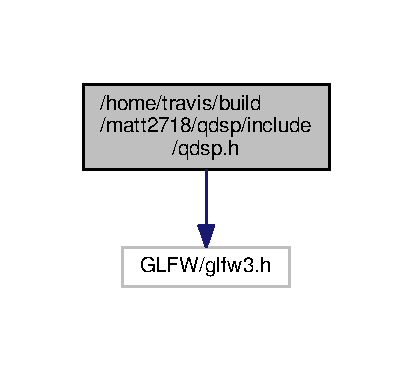
\includegraphics[width=198pt]{qdsp_8h__incl}
\end{center}
\end{figure}
\subsection*{Data Structures}
\begin{DoxyCompactItemize}
\item 
struct \hyperlink{structQDSPplot}{Q\-D\-S\-Pplot}
\end{DoxyCompactItemize}
\subsection*{Typedefs}
\begin{DoxyCompactItemize}
\item 
\hypertarget{qdsp_8h_a3fb39de54c50c78f0ef32c1867a2ef6c}{typedef struct \hyperlink{structQDSPplot}{Q\-D\-S\-Pplot} {\bfseries Q\-D\-S\-Pplot}}\label{qdsp_8h_a3fb39de54c50c78f0ef32c1867a2ef6c}

\end{DoxyCompactItemize}
\subsection*{Functions}
\begin{DoxyCompactItemize}
\item 
\hyperlink{structQDSPplot}{Q\-D\-S\-Pplot} $\ast$ \hyperlink{qdsp_8h_ab48f58716694432ead3ad2aa738dd85d}{qdsp\-Init} (const char $\ast$title)
\begin{DoxyCompactList}\small\item\em Creates a new plot. \end{DoxyCompactList}\item 
void \hyperlink{qdsp_8h_a8b50f4d00f550bbb3b6e50ed0c224f85}{qdsp\-Delete} (\hyperlink{structQDSPplot}{Q\-D\-S\-Pplot} $\ast$plot)
\begin{DoxyCompactList}\small\item\em Destroys a plot. \end{DoxyCompactList}\item 
int \hyperlink{qdsp_8h_a9147cadf7ec7b1d89aa7e2af63d857c2}{qdsp\-Update} (\hyperlink{structQDSPplot}{Q\-D\-S\-Pplot} $\ast$plot, double $\ast$x, double $\ast$y, int $\ast$color, int num\-Points)
\begin{DoxyCompactList}\small\item\em Updates a plot immediately. \end{DoxyCompactList}\item 
int \hyperlink{qdsp_8h_a960f4ed377ad791f7f1ed848e57dbdd7}{qdsp\-Update\-If\-Ready} (\hyperlink{structQDSPplot}{Q\-D\-S\-Pplot} $\ast$plot, double $\ast$x, double $\ast$y, int $\ast$color, int num\-Points)
\begin{DoxyCompactList}\small\item\em Updates a plot if enough time has passed since the last update. \end{DoxyCompactList}\item 
int \hyperlink{qdsp_8h_a743a49615e3853bd2c54f1cbc9e7aae9}{qdsp\-Update\-Wait} (\hyperlink{structQDSPplot}{Q\-D\-S\-Pplot} $\ast$plot, double $\ast$x, double $\ast$y, int $\ast$color, int num\-Points)
\begin{DoxyCompactList}\small\item\em Updates a plot after waiting for a new frame. \end{DoxyCompactList}\item 
void \hyperlink{qdsp_8h_aa96f95a11b1db411dfa77edc1e92c90b}{qdsp\-Redraw} (\hyperlink{structQDSPplot}{Q\-D\-S\-Pplot} $\ast$plot)
\begin{DoxyCompactList}\small\item\em Redraws a plot. \end{DoxyCompactList}\item 
void \hyperlink{qdsp_8h_a6029ae216e906f1d55e2a9815022a93f}{qdsp\-Set\-Framerate} (\hyperlink{structQDSPplot}{Q\-D\-S\-Pplot} $\ast$plot, double framerate)
\begin{DoxyCompactList}\small\item\em Caps the update framerate of a plot. \end{DoxyCompactList}\item 
void \hyperlink{qdsp_8h_a820c950bb4ec854be89ab60b73059d9c}{qdsp\-Set\-Bounds} (\hyperlink{structQDSPplot}{Q\-D\-S\-Pplot} $\ast$plot, double x\-Min, double x\-Max, double y\-Min, double y\-Max)
\begin{DoxyCompactList}\small\item\em Sets the x and y bounds of a plot. \end{DoxyCompactList}\item 
void \hyperlink{qdsp_8h_ad3faa9ad17a6292ee63e6adb5d251219}{qdsp\-Set\-Connected} (\hyperlink{structQDSPplot}{Q\-D\-S\-Pplot} $\ast$plot, int connected)
\begin{DoxyCompactList}\small\item\em Specifies whether to connect the plot points. \end{DoxyCompactList}\item 
void \hyperlink{qdsp_8h_a53adc32f19510e7a7254b5a83f3cc502}{qdsp\-Set\-Point\-Color} (\hyperlink{structQDSPplot}{Q\-D\-S\-Pplot} $\ast$plot, int rgb)
\begin{DoxyCompactList}\small\item\em Sets the default point color. \end{DoxyCompactList}\item 
void \hyperlink{qdsp_8h_a7d4a0c9a9163f95dd71e1110ff8dc200}{qdsp\-Set\-B\-G\-Color} (\hyperlink{structQDSPplot}{Q\-D\-S\-Pplot} $\ast$plot, int rgb)
\begin{DoxyCompactList}\small\item\em Sets the background color. \end{DoxyCompactList}\item 
void \hyperlink{qdsp_8h_a4ef5cd65de47e9b40ee5b1060c801b15}{qdsp\-Set\-Grid\-X} (\hyperlink{structQDSPplot}{Q\-D\-S\-Pplot} $\ast$plot, double point, double interval, int rgb)
\begin{DoxyCompactList}\small\item\em Sets the locations of x gridlines. \end{DoxyCompactList}\item 
void \hyperlink{qdsp_8h_a8ab6e92e54babc386e60134318c273f3}{qdsp\-Set\-Grid\-Y} (\hyperlink{structQDSPplot}{Q\-D\-S\-Pplot} $\ast$plot, double point, double interval, int rgb)
\begin{DoxyCompactList}\small\item\em Sets the locations of y gridlines. \end{DoxyCompactList}\end{DoxyCompactItemize}


\subsection{Detailed Description}
Functions for Q\-D\-S\-P. \begin{DoxyAuthor}{Author}
Matt Mitchell
\end{DoxyAuthor}
This file contains all public function prototypes for Q\-D\-S\-P. 

\subsection{Function Documentation}
\hypertarget{qdsp_8h_a8b50f4d00f550bbb3b6e50ed0c224f85}{\index{qdsp.\-h@{qdsp.\-h}!qdsp\-Delete@{qdsp\-Delete}}
\index{qdsp\-Delete@{qdsp\-Delete}!qdsp.h@{qdsp.\-h}}
\subsubsection[{qdsp\-Delete}]{\setlength{\rightskip}{0pt plus 5cm}void qdsp\-Delete (
\begin{DoxyParamCaption}
\item[{{\bf Q\-D\-S\-Pplot} $\ast$}]{plot}
\end{DoxyParamCaption}
)}}\label{qdsp_8h_a8b50f4d00f550bbb3b6e50ed0c224f85}


Destroys a plot. 

The plot object is freed and all resources are deleted.


\begin{DoxyParams}{Parameters}
{\em plot} & The plot to destroy. \\
\hline
\end{DoxyParams}
\hypertarget{qdsp_8h_ab48f58716694432ead3ad2aa738dd85d}{\index{qdsp.\-h@{qdsp.\-h}!qdsp\-Init@{qdsp\-Init}}
\index{qdsp\-Init@{qdsp\-Init}!qdsp.h@{qdsp.\-h}}
\subsubsection[{qdsp\-Init}]{\setlength{\rightskip}{0pt plus 5cm}{\bf Q\-D\-S\-Pplot}$\ast$ qdsp\-Init (
\begin{DoxyParamCaption}
\item[{const char $\ast$}]{title}
\end{DoxyParamCaption}
)}}\label{qdsp_8h_ab48f58716694432ead3ad2aa738dd85d}


Creates a new plot. 

A new plot is created in a window with the given title.

In order to see a list of plot hotkeys, press 'h' while the plot is running.


\begin{DoxyParams}{Parameters}
{\em title} & The window title.\\
\hline
\end{DoxyParams}
\begin{DoxyReturn}{Returns}
A pointer to the plot handle, or N\-U\-L\-L if a plot could not be created. 
\end{DoxyReturn}
\begin{DoxySeeAlso}{See Also}

\end{DoxySeeAlso}
\hypertarget{qdsp_8h_aa96f95a11b1db411dfa77edc1e92c90b}{\index{qdsp.\-h@{qdsp.\-h}!qdsp\-Redraw@{qdsp\-Redraw}}
\index{qdsp\-Redraw@{qdsp\-Redraw}!qdsp.h@{qdsp.\-h}}
\subsubsection[{qdsp\-Redraw}]{\setlength{\rightskip}{0pt plus 5cm}void qdsp\-Redraw (
\begin{DoxyParamCaption}
\item[{{\bf Q\-D\-S\-Pplot} $\ast$}]{plot}
\end{DoxyParamCaption}
)}}\label{qdsp_8h_aa96f95a11b1db411dfa77edc1e92c90b}


Redraws a plot. 

The given plot is redrawn immediately, ignoring any specified framerate.


\begin{DoxyParams}{Parameters}
{\em plot} & The plot to redraw. \\
\hline
\end{DoxyParams}
\hypertarget{qdsp_8h_a7d4a0c9a9163f95dd71e1110ff8dc200}{\index{qdsp.\-h@{qdsp.\-h}!qdsp\-Set\-B\-G\-Color@{qdsp\-Set\-B\-G\-Color}}
\index{qdsp\-Set\-B\-G\-Color@{qdsp\-Set\-B\-G\-Color}!qdsp.h@{qdsp.\-h}}
\subsubsection[{qdsp\-Set\-B\-G\-Color}]{\setlength{\rightskip}{0pt plus 5cm}void qdsp\-Set\-B\-G\-Color (
\begin{DoxyParamCaption}
\item[{{\bf Q\-D\-S\-Pplot} $\ast$}]{plot, }
\item[{int}]{rgb}
\end{DoxyParamCaption}
)}}\label{qdsp_8h_a7d4a0c9a9163f95dd71e1110ff8dc200}


Sets the background color. 

This function sets the background color of the plot area.


\begin{DoxyParams}{Parameters}
{\em plot} & The plot to act on. \\
\hline
{\em rgb} & The background color, as an integer. Bits 23-\/16 specify the red component, bits 15-\/8 specify the green component, and bits 7-\/0 specify the blue component. All components are interpreted as 8-\/bit unsigned integers.\\
\hline
\end{DoxyParams}
\begin{DoxySeeAlso}{See Also}
\hyperlink{qdsp_8h_a53adc32f19510e7a7254b5a83f3cc502}{qdsp\-Set\-Point\-Color} 
\end{DoxySeeAlso}
\hypertarget{qdsp_8h_a820c950bb4ec854be89ab60b73059d9c}{\index{qdsp.\-h@{qdsp.\-h}!qdsp\-Set\-Bounds@{qdsp\-Set\-Bounds}}
\index{qdsp\-Set\-Bounds@{qdsp\-Set\-Bounds}!qdsp.h@{qdsp.\-h}}
\subsubsection[{qdsp\-Set\-Bounds}]{\setlength{\rightskip}{0pt plus 5cm}void qdsp\-Set\-Bounds (
\begin{DoxyParamCaption}
\item[{{\bf Q\-D\-S\-Pplot} $\ast$}]{plot, }
\item[{double}]{x\-Min, }
\item[{double}]{x\-Max, }
\item[{double}]{y\-Min, }
\item[{double}]{y\-Max}
\end{DoxyParamCaption}
)}}\label{qdsp_8h_a820c950bb4ec854be89ab60b73059d9c}


Sets the x and y bounds of a plot. 

This function sets the bounds of the plot window. The default bounds are (-\/1,-\/1) to (1,1).


\begin{DoxyParams}{Parameters}
{\em plot} & The plot to act on. \\
\hline
{\em x\-Min} & The x coordinate of the plot's left boundary. \\
\hline
{\em x\-Max} & The x coordinate of the plot's right boundary. \\
\hline
{\em y\-Min} & The y coordinate of the plot's lower boundary. \\
\hline
{\em y\-Max} & The y coordinate of the plot's upper boundary. \\
\hline
\end{DoxyParams}
\hypertarget{qdsp_8h_ad3faa9ad17a6292ee63e6adb5d251219}{\index{qdsp.\-h@{qdsp.\-h}!qdsp\-Set\-Connected@{qdsp\-Set\-Connected}}
\index{qdsp\-Set\-Connected@{qdsp\-Set\-Connected}!qdsp.h@{qdsp.\-h}}
\subsubsection[{qdsp\-Set\-Connected}]{\setlength{\rightskip}{0pt plus 5cm}void qdsp\-Set\-Connected (
\begin{DoxyParamCaption}
\item[{{\bf Q\-D\-S\-Pplot} $\ast$}]{plot, }
\item[{int}]{connected}
\end{DoxyParamCaption}
)}}\label{qdsp_8h_ad3faa9ad17a6292ee63e6adb5d251219}


Specifies whether to connect the plot points. 

This function tells Q\-D\-S\-P whether the points in the specified plot should be disconnected (to draw a scatter plot) or connected (to draw a line plot).


\begin{DoxyParams}{Parameters}
{\em plot} & The plot to act on. \\
\hline
{\em connected} & Zero if the points should be disconnected, nonzero if they should be connected. \\
\hline
\end{DoxyParams}
\hypertarget{qdsp_8h_a6029ae216e906f1d55e2a9815022a93f}{\index{qdsp.\-h@{qdsp.\-h}!qdsp\-Set\-Framerate@{qdsp\-Set\-Framerate}}
\index{qdsp\-Set\-Framerate@{qdsp\-Set\-Framerate}!qdsp.h@{qdsp.\-h}}
\subsubsection[{qdsp\-Set\-Framerate}]{\setlength{\rightskip}{0pt plus 5cm}void qdsp\-Set\-Framerate (
\begin{DoxyParamCaption}
\item[{{\bf Q\-D\-S\-Pplot} $\ast$}]{plot, }
\item[{double}]{framerate}
\end{DoxyParamCaption}
)}}\label{qdsp_8h_a6029ae216e906f1d55e2a9815022a93f}


Caps the update framerate of a plot. 

This function sets a framerate for updating the specified plot, which will be used by \hyperlink{qdsp_8h_a960f4ed377ad791f7f1ed848e57dbdd7}{qdsp\-Update\-If\-Ready} and \hyperlink{qdsp_8h_a743a49615e3853bd2c54f1cbc9e7aae9}{qdsp\-Update\-Wait}. If the specified framerate is less than or equal to 0, the framerate will be uncapped and the aforementioned functions will behave like \hyperlink{qdsp_8h_a9147cadf7ec7b1d89aa7e2af63d857c2}{qdsp\-Update} when called.

The default framerate is 60 F\-P\-S.


\begin{DoxyParams}{Parameters}
{\em plot} & The plot to act on. \\
\hline
{\em framerate} & The framerate, in frames per second.\\
\hline
\end{DoxyParams}
\begin{DoxySeeAlso}{See Also}
\hyperlink{qdsp_8h_a960f4ed377ad791f7f1ed848e57dbdd7}{qdsp\-Update\-If\-Ready} 

\hyperlink{qdsp_8h_a743a49615e3853bd2c54f1cbc9e7aae9}{qdsp\-Update\-Wait} 
\end{DoxySeeAlso}
\hypertarget{qdsp_8h_a4ef5cd65de47e9b40ee5b1060c801b15}{\index{qdsp.\-h@{qdsp.\-h}!qdsp\-Set\-Grid\-X@{qdsp\-Set\-Grid\-X}}
\index{qdsp\-Set\-Grid\-X@{qdsp\-Set\-Grid\-X}!qdsp.h@{qdsp.\-h}}
\subsubsection[{qdsp\-Set\-Grid\-X}]{\setlength{\rightskip}{0pt plus 5cm}void qdsp\-Set\-Grid\-X (
\begin{DoxyParamCaption}
\item[{{\bf Q\-D\-S\-Pplot} $\ast$}]{plot, }
\item[{double}]{point, }
\item[{double}]{interval, }
\item[{int}]{rgb}
\end{DoxyParamCaption}
)}}\label{qdsp_8h_a4ef5cd65de47e9b40ee5b1060c801b15}


Sets the locations of x gridlines. 

This function determines the spacing of the x gridlines. Gridlines will be spaced the given interval apart, with one gridline placed exactly at the given point.


\begin{DoxyParams}{Parameters}
{\em plot} & The plot to act on. \\
\hline
{\em point} & A specific x-\/coordinate that a gridline should be placed at. All gridlines will be placed an integer multiple of the specified interval from this position. \\
\hline
{\em interval} & The distance between gridlines. \\
\hline
{\em rgb} & The point color. See \hyperlink{qdsp_8h_a7d4a0c9a9163f95dd71e1110ff8dc200}{qdsp\-Set\-B\-G\-Color} for a description of the color format.\\
\hline
\end{DoxyParams}
\begin{DoxySeeAlso}{See Also}
\hyperlink{qdsp_8h_a8ab6e92e54babc386e60134318c273f3}{qdsp\-Set\-Grid\-Y} 
\end{DoxySeeAlso}
\hypertarget{qdsp_8h_a8ab6e92e54babc386e60134318c273f3}{\index{qdsp.\-h@{qdsp.\-h}!qdsp\-Set\-Grid\-Y@{qdsp\-Set\-Grid\-Y}}
\index{qdsp\-Set\-Grid\-Y@{qdsp\-Set\-Grid\-Y}!qdsp.h@{qdsp.\-h}}
\subsubsection[{qdsp\-Set\-Grid\-Y}]{\setlength{\rightskip}{0pt plus 5cm}void qdsp\-Set\-Grid\-Y (
\begin{DoxyParamCaption}
\item[{{\bf Q\-D\-S\-Pplot} $\ast$}]{plot, }
\item[{double}]{point, }
\item[{double}]{interval, }
\item[{int}]{rgb}
\end{DoxyParamCaption}
)}}\label{qdsp_8h_a8ab6e92e54babc386e60134318c273f3}


Sets the locations of y gridlines. 

This function determines the spacing of the y gridlines. Gridlines will be spaced the given interval apart, with one gridline placed exactly at the given point.


\begin{DoxyParams}{Parameters}
{\em plot} & The plot to act on. \\
\hline
{\em point} & A specific y-\/coordinate that a gridline should be placed at. All gridlines will be placed an integer multiple of the specified interval from this position. \\
\hline
{\em interval} & The distance between gridlines. \\
\hline
{\em rgb} & The point color. See \hyperlink{qdsp_8h_a7d4a0c9a9163f95dd71e1110ff8dc200}{qdsp\-Set\-B\-G\-Color} for a description of the color format.\\
\hline
\end{DoxyParams}
\begin{DoxySeeAlso}{See Also}
\hyperlink{qdsp_8h_a4ef5cd65de47e9b40ee5b1060c801b15}{qdsp\-Set\-Grid\-X} 
\end{DoxySeeAlso}
\hypertarget{qdsp_8h_a53adc32f19510e7a7254b5a83f3cc502}{\index{qdsp.\-h@{qdsp.\-h}!qdsp\-Set\-Point\-Color@{qdsp\-Set\-Point\-Color}}
\index{qdsp\-Set\-Point\-Color@{qdsp\-Set\-Point\-Color}!qdsp.h@{qdsp.\-h}}
\subsubsection[{qdsp\-Set\-Point\-Color}]{\setlength{\rightskip}{0pt plus 5cm}void qdsp\-Set\-Point\-Color (
\begin{DoxyParamCaption}
\item[{{\bf Q\-D\-S\-Pplot} $\ast$}]{plot, }
\item[{int}]{rgb}
\end{DoxyParamCaption}
)}}\label{qdsp_8h_a53adc32f19510e7a7254b5a83f3cc502}


Sets the default point color. 

This function sets the point color to use when no color array is specified during an update.


\begin{DoxyParams}{Parameters}
{\em plot} & The plot to act on. \\
\hline
{\em rgb} & The point color. See \hyperlink{qdsp_8h_a7d4a0c9a9163f95dd71e1110ff8dc200}{qdsp\-Set\-B\-G\-Color} for a description of the color format.\\
\hline
\end{DoxyParams}
\begin{DoxySeeAlso}{See Also}
\hyperlink{qdsp_8h_a7d4a0c9a9163f95dd71e1110ff8dc200}{qdsp\-Set\-B\-G\-Color} 
\end{DoxySeeAlso}
\hypertarget{qdsp_8h_a9147cadf7ec7b1d89aa7e2af63d857c2}{\index{qdsp.\-h@{qdsp.\-h}!qdsp\-Update@{qdsp\-Update}}
\index{qdsp\-Update@{qdsp\-Update}!qdsp.h@{qdsp.\-h}}
\subsubsection[{qdsp\-Update}]{\setlength{\rightskip}{0pt plus 5cm}int qdsp\-Update (
\begin{DoxyParamCaption}
\item[{{\bf Q\-D\-S\-Pplot} $\ast$}]{plot, }
\item[{double $\ast$}]{x, }
\item[{double $\ast$}]{y, }
\item[{int $\ast$}]{color, }
\item[{int}]{num\-Points}
\end{DoxyParamCaption}
)}}\label{qdsp_8h_a9147cadf7ec7b1d89aa7e2af63d857c2}


Updates a plot immediately. 

The plot is updated with the new vertex data and immediately redrawn, ignoring any specified framerate. If color is N\-U\-L\-L, all points will be the default color.

\hyperlink{qdsp_8h_a960f4ed377ad791f7f1ed848e57dbdd7}{qdsp\-Update\-If\-Ready} should be preferred in many cases, as repeated calls to qdsp\-Update per frame will result in a lot of useless overhead.


\begin{DoxyParams}{Parameters}
{\em plot} & The plot to update. \\
\hline
{\em x} & An array containing the x coordinates. \\
\hline
{\em y} & An array containing the y coordinates. \\
\hline
{\em color} & An array containing the point colors, or N\-U\-L\-L. See \hyperlink{qdsp_8h_a7d4a0c9a9163f95dd71e1110ff8dc200}{qdsp\-Set\-B\-G\-Color} for a description of the color format. \\
\hline
{\em num\-Points} & The number of points to render.\\
\hline
\end{DoxyParams}
\begin{DoxyReturn}{Returns}
1 if the plot was updated successfully, 0 otherwise.
\end{DoxyReturn}
\begin{DoxySeeAlso}{See Also}
\hyperlink{qdsp_8h_a960f4ed377ad791f7f1ed848e57dbdd7}{qdsp\-Update\-If\-Ready} 

\hyperlink{qdsp_8h_a743a49615e3853bd2c54f1cbc9e7aae9}{qdsp\-Update\-Wait} 

\hyperlink{qdsp_8h_aa96f95a11b1db411dfa77edc1e92c90b}{qdsp\-Redraw} 
\end{DoxySeeAlso}
\hypertarget{qdsp_8h_a960f4ed377ad791f7f1ed848e57dbdd7}{\index{qdsp.\-h@{qdsp.\-h}!qdsp\-Update\-If\-Ready@{qdsp\-Update\-If\-Ready}}
\index{qdsp\-Update\-If\-Ready@{qdsp\-Update\-If\-Ready}!qdsp.h@{qdsp.\-h}}
\subsubsection[{qdsp\-Update\-If\-Ready}]{\setlength{\rightskip}{0pt plus 5cm}int qdsp\-Update\-If\-Ready (
\begin{DoxyParamCaption}
\item[{{\bf Q\-D\-S\-Pplot} $\ast$}]{plot, }
\item[{double $\ast$}]{x, }
\item[{double $\ast$}]{y, }
\item[{int $\ast$}]{color, }
\item[{int}]{num\-Points}
\end{DoxyParamCaption}
)}}\label{qdsp_8h_a960f4ed377ad791f7f1ed848e57dbdd7}


Updates a plot if enough time has passed since the last update. 

The plot is updated with the new vertex data and redrawn if at least 1.\-0/framerate seconds have passed since the last call to \hyperlink{qdsp_8h_a9147cadf7ec7b1d89aa7e2af63d857c2}{qdsp\-Update}, \hyperlink{qdsp_8h_a960f4ed377ad791f7f1ed848e57dbdd7}{qdsp\-Update\-If\-Ready}, \hyperlink{qdsp_8h_a743a49615e3853bd2c54f1cbc9e7aae9}{qdsp\-Update\-Wait}, or \hyperlink{qdsp_8h_aa96f95a11b1db411dfa77edc1e92c90b}{qdsp\-Redraw} in which the specified plot was redrawn. If color is N\-U\-L\-L, all points will be the default color.

This function should be used over \hyperlink{qdsp_8h_a9147cadf7ec7b1d89aa7e2af63d857c2}{qdsp\-Update} in many cases, as it eliminates the useless overhead of copying vertex data to the G\-P\-U before the monitor can be refreshed.


\begin{DoxyParams}{Parameters}
{\em plot} & The plot to update. \\
\hline
{\em x} & An array containing the x coordinates. \\
\hline
{\em y} & An array containing the y coordinates. \\
\hline
{\em color} & An array containing the point colors, or N\-U\-L\-L. See \hyperlink{qdsp_8h_a7d4a0c9a9163f95dd71e1110ff8dc200}{qdsp\-Set\-B\-G\-Color} for a description of the color format. \\
\hline
{\em num\-Points} & The number of points to render.\\
\hline
\end{DoxyParams}
\begin{DoxyReturn}{Returns}
1 if the plot was updated successfully, 2 if plot was not ready for an update, 0 otherwise.
\end{DoxyReturn}
\begin{DoxySeeAlso}{See Also}
\hyperlink{qdsp_8h_a9147cadf7ec7b1d89aa7e2af63d857c2}{qdsp\-Update} 

\hyperlink{qdsp_8h_a743a49615e3853bd2c54f1cbc9e7aae9}{qdsp\-Update\-Wait} 

\hyperlink{qdsp_8h_aa96f95a11b1db411dfa77edc1e92c90b}{qdsp\-Redraw} 

\hyperlink{qdsp_8h_a6029ae216e906f1d55e2a9815022a93f}{qdsp\-Set\-Framerate} 
\end{DoxySeeAlso}
\hypertarget{qdsp_8h_a743a49615e3853bd2c54f1cbc9e7aae9}{\index{qdsp.\-h@{qdsp.\-h}!qdsp\-Update\-Wait@{qdsp\-Update\-Wait}}
\index{qdsp\-Update\-Wait@{qdsp\-Update\-Wait}!qdsp.h@{qdsp.\-h}}
\subsubsection[{qdsp\-Update\-Wait}]{\setlength{\rightskip}{0pt plus 5cm}int qdsp\-Update\-Wait (
\begin{DoxyParamCaption}
\item[{{\bf Q\-D\-S\-Pplot} $\ast$}]{plot, }
\item[{double $\ast$}]{x, }
\item[{double $\ast$}]{y, }
\item[{int $\ast$}]{color, }
\item[{int}]{num\-Points}
\end{DoxyParamCaption}
)}}\label{qdsp_8h_a743a49615e3853bd2c54f1cbc9e7aae9}


Updates a plot after waiting for a new frame. 

This function waits until at least 1.\-0/framerate seconds have passed since the last call to \hyperlink{qdsp_8h_a9147cadf7ec7b1d89aa7e2af63d857c2}{qdsp\-Update}, \hyperlink{qdsp_8h_a960f4ed377ad791f7f1ed848e57dbdd7}{qdsp\-Update\-If\-Ready}, \hyperlink{qdsp_8h_a743a49615e3853bd2c54f1cbc9e7aae9}{qdsp\-Update\-Wait}, or \hyperlink{qdsp_8h_aa96f95a11b1db411dfa77edc1e92c90b}{qdsp\-Redraw} in which the specified plot was redrawn. It then updates the plot with the vertex data and redraws it. If color is N\-U\-L\-L, all points will be the default color.

This function is primarily useful when you wish to limit your code to a specific real-\/time update interval.


\begin{DoxyParams}{Parameters}
{\em plot} & The plot to update. \\
\hline
{\em x} & An array containing the x coordinates. \\
\hline
{\em y} & An array containing the y coordinates. \\
\hline
{\em color} & An array containing the point colors, or N\-U\-L\-L. See \hyperlink{qdsp_8h_a7d4a0c9a9163f95dd71e1110ff8dc200}{qdsp\-Set\-B\-G\-Color} for a description of the color format. \\
\hline
{\em num\-Points} & The number of points to render.\\
\hline
\end{DoxyParams}
\begin{DoxyReturn}{Returns}
1 if the plot was updated successfully, 0 otherwise.
\end{DoxyReturn}
\begin{DoxySeeAlso}{See Also}
\hyperlink{qdsp_8h_a9147cadf7ec7b1d89aa7e2af63d857c2}{qdsp\-Update} 

\hyperlink{qdsp_8h_a960f4ed377ad791f7f1ed848e57dbdd7}{qdsp\-Update\-If\-Ready} 

\hyperlink{qdsp_8h_aa96f95a11b1db411dfa77edc1e92c90b}{qdsp\-Redraw} 

\hyperlink{qdsp_8h_a6029ae216e906f1d55e2a9815022a93f}{qdsp\-Set\-Framerate} 
\end{DoxySeeAlso}

%--- End generated contents ---

% Index
\newpage
\phantomsection
\addcontentsline{toc}{chapter}{Index}
\printindex

\end{document}
